\chapter{Técnicas}

\section{Test-Driven Development (TDD)}
\label{sec:tdd}
``Apenas escrever código para corrigir um teste falhando". Segundo \citeonline{TestDrivenKoskela}, isto é \textit{Test-Driven Development} (Desenvolvimento guiado por testes) \cite{TDDbyExample} em apenas uma sentença.

O TDD é uma técnica onde o desenvolvimento do software é guiado por \textbf{testes automatizados}, que são escritos antes de qualquer linha de código relativo a funcionalidades. Primeiro escreve-se um teste, depois escreve-se o código para passar neste teste. Em seguida, o código é refatorado para encontrar um design melhor, contando sempre com os testes existentes para que não sejam introduzidas falhas em outras partes do sistema.

Esta abordagem encoraja bom design \cite{GrowingOOByTests}, produz código testável e mantém longe a sobre-engenharia por conta de falsas suposições, pois, nos testes, é especificado o que é desejado e escreve-se o código para fazer apenas aquilo que realmente é necessário. \cite{TestDrivenKoskela, TDDbyExample, EmpiricalTDD}

\citeonline{EmergentDesign} coloca de maneira interessante a relação entre o entendimento do problema e o fluxo natural do TDD:

\begin{citacao}
Tentar escrever um teste é uma boa maneira de testar a si mesmo sobre seu conhecimento sobre como a classe deverá funcionar antes de você escrevê-la. Esta é uma boa sequência: tenha certeza de que você entende o que você irá tentar fazer antes de você realmente tentar fazer. De fato, colocando dessa maneira parece muito mais natural considerar os testes como Primeira Tarefa e criar o código como Segunda Tarefa. (tradução do autor)
\end{citacao}

Mas TDD é uma técnica emergente? Não e sim.

O TDD vem sendo utilizado esporadicamente há anos, contudo, não existia um nome para identificar essa forma de desenvolver software. Atualmente, esta técnica tem uma definição, um nome e começa a ganhar força, sendo utilizada em times de grandes empresas como Google, Yahoo, Microsoft e IBM \cite{EmpiricalTDD}.

\subsection{Ciclo TDD}
\label{ssub:ciclo_tdd}

Com base no trabalho de \citeonline{TDDbyExample}, o ciclo de desenvolvimento TDD é composto pelas seguintes etapas:

\begin{enumerate}
\item \textbf{Adicionar um teste}

Cada ciclo se inicia com a criação de um teste de unidade. Este teste inevitavelmente irá falhar, pois é escrito antes do código ser implementado de fato. Para escrever um teste, o desenvolvedor precisa entender claramente as especificações e requisitos da unidade. Isso faz com que o desenvolvedor tenha como foco os requisitos antes do código, o direcionando a escrever código apenas para o que é realmente necessário.

\item \textbf{Executar todos os testes e ver se algum falha}

Todos os testes devem ser executados e o novo teste deve falhar pela razão esperada: a funcionalidade não foi desenvolvida. Isto aumenta a confiança que se está testando a coisa certa.

\item \textbf{Escrever código}

O próximo passo é escrever código \textbf{somente para que o teste passe}. O código poderá não ser perfeito, pois posteriormente ele será melhorado. O importante é que o código faça o mínimo para passar no teste. Segundo \citeonline{BDDRodrigo}:

\begin{citacao}
Enquanto código útil é um patrimônio que gera valor, qualquer código criado inutilmente é tempo desperdiçado e, no fim das contas, um fardo, que sem gerar valor algum, aumentará a complexidade geral do software.
\end{citacao}

\item \textbf{Executar os testes e ter sucesso}

Ao Executar os testes e todos eles passarem, o código possuirá todos os requisitos testados e o programador pode ficar confiante para melhorá-lo.

\item \textbf{Refatorar}

Esta é uma etapa muito importante, onde o código escrito anteriormente é melhorado.

Segundo \citeonline{FowlerRefatoracao}, refatorar é reestruturar o software aplicando uma série de alterações em sua estrutura interna para torná-lo mais fácil de ser entendido e menos custoso de ser modificado, sem alterar seu comportamento observável.

Refatorar melhora o projeto do software, o torna mais fácil de entender e modificar, ajuda a encontrar falhas e ajuda o desenvolvedor a programar mais rapidamente.

Como na refatoração o comportamento do código não deve ser alterado, após refatorar e executar novamente os testes, todos eles devem passar.

\end{enumerate}

A figura \ref{img:ciclo-tdd} resume o ciclo TDD de forma bem clara.

\begin{figure}[h]
  \center
  \caption{O ciclo TDD}
  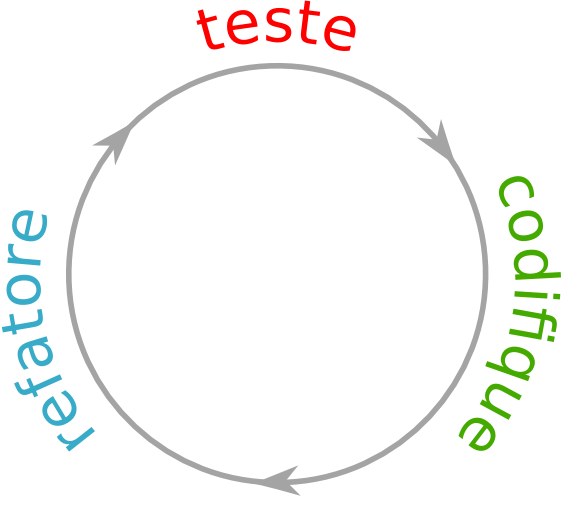
\includegraphics[scale=0.45]{images/ciclo-tdd}
  \label{img:ciclo-tdd}
\end{figure}

\subsection{TDD na prática}
\label{ssub:tdd_na_pratica}

Neste subtópico será apresentada como a utilização do TDD se dá na prática, utilizando exemplos reais implementados durante do desenvolvimento do kanban-roots.

A seguinte funcionalidade precisa ser implementada:

\begin{quote}
\textit{Precisa-se saber todas as tarefas em uma determinada posição do kanban (quadro) de um projeto.}
\end{quote}

A primeira coisa a ser feita é o teste para o caso mais simples: quando o projeto não tem tarefa alguma naquela determinada posição do kanban.

Desta forma, o teste para o caso mais simples pode ser como mostrado no Código \ref{code:tdd_test1}.

\begin{mycode}{ruby}%
{Teste para o método Project\#tasks\_by\_position (versão 1)}{code:tdd_test1}
# test/unit/project_test.rb
class ProjectTest < ActiveSupport::TestCase
  def test_tasks_by_position
    project = Factory.create :project
    assert_equal(project.tasks_by_position(4), [])
  end
end
\end{mycode}

Ao rodar este teste, ele irá falhar, informando que o método \texttt{tasks\_by\_position} sequer existe. Como esta era a falha esperada, é escrito então o código mais simples para passar neste teste, apresentado no Código \ref{code:tdd_code1}.

\begin{mycode}{ruby}%
{Código do método Project\#tasks\_by\_position (versão 1)}{code:tdd_code1}
# app/models/project.rb
def tasks_by_position position
  []
end
\end{mycode}

Os testes irão passar. Mas a funcionalidade ainda não está completa e, consequentemente, o teste também não. Como pode ser visto no Código \ref{code:tdd_test2}, é adicionado ao teste uma verificação de que para a posição 1 devem existir duas tarefas e que estas tarefas devem ser exatamente as criadas anteriormente.

\begin{mycode}{ruby}%
{Teste do método Project\#tasks\_by\_position (versão 2)}{code:tdd_test2}
# test/unit/project_test.rb
class ProjectTest < ActiveSupport::TestCase
  def test_tasks_by_position
    project = Factory.create :project
    tasks = [Factory.create(:task, :project => project, :position => 1),
             Factory.create(:task, :project => project, :position => 1)]

    assert_equal(project.tasks_by_position(4), [])

    assert_equal(project.tasks_by_position(1).count, 2)
    tasks.each { |task| assert(project.tasks_by_position(1).include?(task)) }
  end
end
\end{mycode}

Como o teste foi alterado, este é executado e irá falhar, informando que na \hyperref[code:tdd_test2]{linha 10} eram esperadas duas tarefas, mas foram obtidas zero. O código então deve ser modificado para passar no novo teste e é apresentado no código \ref{code:tdd_code2}.

\begin{mycode}{ruby}%
{Código do método Project\#tasks\_by\_position (versão 2)}{code:tdd_code2}
# app/models/project.rb
def tasks_by_position position
  task_list = []
  tasks.each do |task|
    task_list << task if task.position.to_s == position.to_s
  end
  task_list
end
\end{mycode}

Desta vez, após a modificação no código e a execução dos testes, todos os testes os irão passar. Contudo, a cobertura de testes para este método ainda está fraca, o que pode ser resolvido com a adição de mais algumas tarefas em posições diferentes, como mostrado no Código \ref{code:tdd_test3}.

\begin{mycode}{ruby}%
{Teste do método Project\#tasks\_by\_position (versão 3)}{code:tdd_test3}
# test/unit/project_test.rb
class ProjectTest < ActiveSupport::TestCase
  def test_tasks_by_position
    project = Factory.create :project
    tasks = [Factory.create(:task, :project => project, :position => 1),
             Factory.create(:task, :project => project, :position => 1),
             Factory.create(:task, :project => project, :position => 2),
             Factory.create(:task, :project => project, :position => 3),
             Factory.create(:task, :project => project, :position => 3)]

    assert_equal(project.tasks_by_position(4), [])

    assert_equal(project.tasks_by_position(1).count, 2)
    tasks[0..1].each { |task| assert(project.tasks_by_position(1).include?(task)) }

    assert_equal(project.tasks_by_position(2), [tasks[2]])

    assert_equal(project.tasks_by_position("3").count, 2)
    tasks[3..4].each { |task| assert(project.tasks_by_position("3").include?(task)) }
  end
end
\end{mycode}

Executando os testes novamente, todos eles passam. Isto indica que já é hora de ir para o item 5 do ciclo TDD e refatorar. Ao comparar o Código \ref{code:tdd_code2} com sua versão refatorada, apresentada no Código \ref{code:tdd_code3}, pode-se perceber como a segunda está mais simples e clara e que ao rodar os testes, estes passam mostrando que o comportamento do método não mudou.

\begin{mycode}{ruby}%
{Código do método Project\#tasks\_by\_position (versão 3)}{code:tdd_code3}
# app/models/project.rb
def tasks_by_position position
  tasks.select { |item| item.position.to_s == position.to_s }
end
\end{mycode}

Com isso, o ciclo TDD o desenvolvimento da funcionalidade é terminado, produzindo um código legível, limpo e bem coberto por testes.

\subsection{Design emergente} % (fold)
\label{sub:design_emergente}

No contexto em que TDD costuma ser aplicado $-$ em processos ágeis, com um ciclo de vida iterativo-incremental $-$ não é realizado um amplo \textit{design} prévio. Sendo assim, o \textit{design} evolui incrementalmente. Sabendo disso, uma característica extremamente importante do TDD é a facilitação ao \textit{design} emergente, que muitos consideram ser sua a principal característica \cite{EmergentDesign}.

TDD é considerada uma técnica essencial para o \textit{design} emergente porque
quando se está escrevendo um teste anteriormente ao código, o programador contempla e decide não apenas a interface do software (i.e. nomes de classes/métodos, parâmetros, tipos de retorno, lançamento de exceções), mas também o comportamento do software (i.e. resultados esperados para determinadas entradas) \cite{JanzenTDD}.

Além disso, \citeonline{EmergentDesign} constata que o ponto de vista do teste pode passar informações sobre o design, porque o teste de uma classe funciona como o primeiro cliente da classe. Com isso, a interface que o teste sugere é uma interface dirigida ao cliente, sendo assim, geralmente é mais estável.

\citeonline{DammTDD} também afirmam que o TDD faz com que as pessoas pensem mais no design em vez de codificar precipitadamente sem saber o que implementar ainda e \citeonline{XPTeles} ressalta a importância da \textit{refatoração} para a evolução incremental do design:

\begin{citacao}
Ao longo das iterações, o design precisa evoluir, mas deve manter-se simples e claro para que a equipe possa fazer alterações no software a qualquer momento, com facilidade. Por esta razão o \textit{refactoring} tem um papel fundamental no design.
\end{citacao}

\subsubsection{Design emergente no kanban-roots} % (fold)
\label{ssub:design_emergente_no_kanban_roots}

Para o desenvolvimento do kanban-roots, foi de extrema importância que o design evoluísse incrementalmente, pois não se sabia ao certo que funcionalidades seriam contempladas nem que entidades existiriam.

As entidades \textit{Projects} e \textit{Contributors} tinham uma relação direta. Em um dado momento, achou-se pertinente a criação de uma nova entidade \textit{Team} que faria a ligação entre as outras duas entidades. Isto acarretou um uma série de alterações na interface das entidades, na estrutura do banco de dados e etc \cite{CommitAddTeam}. Meses depois, foi verificado que esta entidade \textit{Team} não era mais necessária, acarretando novamente em diversas modificações \cite{CommitRemoveTeam}.

Em uma outra situação, percebeu-se a necessidade do usuário (\textit{Contributor}) ter um \textit{username}, que seria utilizado, entre outras coisas, para fazer o login antes feito apenas com a utilização do email. Para isso, foram feitas algumas modificações no código existente, para que esse suporte fosse adicionado \cite{CommitAddUsername}.

Foram diversas as situações em que mudanças como essa ocorreram durante o desenvolvimento do kanban-roots. Sem o suporte do TDD seria extremamente complicado fazer essas alterações e deixar o design emergir, pois a insegurança de que as modificações pudesse afetar outras partes do código seria muito grande. Além disso, a criação a priore dos testes favoreceu que as modificações fossem feitas de maneira mais simples e direta.

% subsubsection design_emergente_no_kanban_roots (end)

% subsection design_emergente (end)

\subsection{Usar TDD sempre?} % (fold)
\label{sec:usar_tdd_sempre}

Existe um debate sobre a não utilização do TDD em qualquer situação. É dito ``sobre a \textbf{não} utilização"\ pois o autor desconhece qualquer literatura dizendo que TDD deve ser utilizado sempre e em qualquer situação. Na realidade, o que existe é um mal entendido na comunidade sobre o que que alguns ``Agile Experts"\ dizem.

\citeonline{CleanCode}, considerado um ``Agile Expert", define As Três Leis do TDD, onde a primeira delas é: ``Você não pode escrever código de produção até que você tenha escrito um teste de unidade com falha.". O que parece é que fecha-se os olhos para o trecho ``de produção", distorcendo completamente seu sentido.

\citeonline{TDDGiveMeABreak} questiona a posição do que ele chama de ``Agile Testing Experts":

\begin{citacao}
Exigir que você sempre deve escrever os testes primeiro? Dá um tempo. Isso é idiotice em fase de projeto, de hacking, ou de descobertas.

Fazer com que testar seja uma parte central do processo porque eles são úteis para os desenvolvedores? Muito bom. Ditar um fluxo de trabalho para os desenvolvedores que funciona em alguns casos como O Único Caminho Verdadeiro: ridículo.

Testar é ajudar os desenvolvedores, e deve-se reconhecer que o teste automatizado são para benefício dos desenvolvedores, ao invés de \textit{cargo-culting}\footnote{O termo cargo-culting é utilizando quando um programador não qualificados ou iniciante (ou não experiência com o problema em mãos) copia um código de um lugar e colá-o em outro, com pouco ou nenhum entendimento de como o código funciona, ou se é realmente exigido na sua nova posição \cite{CargoCulting}.} um fluxo de trabalho e decretando que ``um tamanho de sapato serve para todos os tipos de pés". (tradução do autor)
\end{citacao}

Já \citeonline{ChromaticTDD} é um pouco mais moderado e diz:

\begin{citacao}
Se eu nunca usei a API antes, TDD pode não ser adequado. Se eu nunca vou usar o código novamente, TDD pode não ser adequado. Se leva mais tempo para escrever os testes (Nove linhas de código no programa final? Provavelmente não vale a pena agora.) do que para escrever e executar o código, TDD pode não ser adequado. (tradução do autor)
\end{citacao}

Introduzindo o kanban-roots na discussão, nos dois únicos casos em que ocorreu um \textit{bug} em produção, ao ser feita uma analise no código em busca da solução, foi encontrado um comentário ``TODO: test it!"\ nos métodos onde os \textit{bugs} ocorreram. Atualmente, existem 13 comentários como esse espalhados no código do kanban-roots. Isso, de certa forma, comprava que caso os testes não sejam escritos antes, para um código que irá entrar em produção, escrevê-lo depois acaba sendo um fardo, e isso é ignorado até que um problema ocorra.

Um exemplo para esta situação é apresentado no código \ref{code:gravatar} que implementa a captura da foto do usuário no kanban-roots. Esta imagem é capturada de um serviço, externo à aplicação, chamado Gravatar\footnote{Serviço que permite a associação de um avatar (imagem) à uma endereço de email. Mais informações em \url{http://gravatar.com}}. Este foi um típico caso onde um experimento foi para produção, sem testes e com o agravante de envolver um serviço externo. Isso porque, apesar de não ser uma boa prática, o Gravatar modificar sua API. Além disso, o Gravatar pode estar indisponível. Não existe nenhum teste para esse método e, principalmente, um teste de integração, que é indispensável nesse caso, foi totalmente negligenciado.

\begin{mycode}{ruby}%
{Código do método que recupera a imagem do Gravatar}{code:gravatar}
# app/helpers/application_helper.rb
# TODO: Test it!
def gravatar_image_tag(user, options={})
  options.reverse_merge!(:size => 24, :class => '')
  if Rails.env.production?
    gravatar_id = Digest::MD5.hexdigest(user.email.downcase)
    url = "http://gravatar.com/avatar/#{gravatar_id}?d=mm&s=#{options[:size]}"
    image_tag(url,
              :class => "avatar #{options[:class]}",
              :height => options[:size],
              :width => options[:size]).html_safe
  else
    image_tag('gravatar.png',
              :class => "avatar #{options[:class]}",
              :height => options[:size],
              :width => options[:size]).html_safe
  end
end
\end{mycode}

\citeonline{LegacyCode} define que \textbf{código legado é código sem testes}. Esta afirmação, que pode parecer extremada, é simplesmente a constatação de que, sem uma ampla cobertura de testes automatizados, e uma vez que é economicamente inviável a aplicação manual de todos os casos de teste $-$ ou mesmo de parte deles $-$ de um software a cada modificação, é muito difícil ter uma margem razoável de segurança de que uma modificação não irá introduzir \textit{bugs} no software. Deste modo, para um código ``que irá para produção"\ a utilização do TDD é essencial, pois do contrário, se está criando código legado. É importante lembrar que o código legado com o tempo vai minando a manutenibilidade do sistema e assim, elevando os custos de introdução de novas funcionalidade e evolução do mesmo.

O autor considera que somente para casos em que um código é apenas prova de conceito ou experimento, e que será eliminado, a utilização da técnica não é invariavelmente necessária. Contudo, a utilização de TDD nesses cenários pode ser muito interessante, pois como dito anteriormente, para a escrita dos testes, é preciso entender bem o problema a ser resolvido, fazendo o desenvolvedor se preparar mais para o que ele ainda não conhece muito bem.

% subsection usar_tdd_sempre (end)

\subsection{TDD realmente é efetivo?} % (fold)
\label{sub:tdd_realmente_e_efetivo}

Existem dúvidas sobre a real efetividade do TDD no que diz respeito à qualidade do código, redução de defeitos e ao aumento ou diminuição da produtividade. Geralmente esta dúvida surge em que nunca realmente praticou TDD. Contudo, por ser um processo complexo, é muito difícil avaliar e chegar a uma conclusão exata sobre os ganhos e benefícios de toda e qualquer prática em engenharia de software.

Nos últimos anos, vem sendo feitos alguns experimentos para tentar mostrar de maneira empírica que TDD realmente é efetivo no processo de desenvolvimento de software.

\subsubsection{Estudos na indústria} % (fold)
\label{sub:estudos_na_industria}

Um estudo feito por \citeonline{MaximilienTDD}, fazendo um comparativo de entre o desenvolvimento pré e pós a utilização do TDD, mostrou uma redução de 50\% na taxa de defeitos encontrados no sistema, tendo um mínimo impacto negativo na produtividade da equipe. Além disso, foi percebido que a utilização do TDD os fez produzir um produto que incorporaria mais facilmente alterações posteriores.

Outro estudo feito por \citeonline{ChinaTDD} dividiu dois grupos, um utilizando TDD e outro utilizando Test-last\footnote{Nesta abordagem os testes escritos após o código.}. O estudo mostrou que o time que utilizou TDD produziu menos defeitos e quando estes ocorriam, eram capazes de solucioná-los muito mais rapidamente. No estudo realizado por \citeonline{DammTDD} também é mostrada uma redução nas taxas de defeito.

Já o estudo feito por \citeonline{GeorgeTDD} mostrou que, apesar de TDD poder reduzir inicialmente a produtividade dos desenvolvedores em 16\%, o código produzido apresentou uma cobertura entre 92\% a 98\%. Além disso, uma análise qualitativa mostrou que 87.5\% dos programadores acreditam que TDD facilitou o entendimento dos requisitos e 95.8\% acreditam que TDD reduziu o tempo gasto com debug. 78\% também acreditam que TDD aumentou a produtividade da equipe. No entanto, apenas metade dos desenvolvedores acreditam que TDD leva a uma diminuição do tempo de desenvolvimento. Sobre qualidade, 92\% acreditam que TDD ajuda a manter um código de maior qualidade e 79\% acreditam que ele promove um design mais simples e 71\% acreditam que esta abordagem é notavelmente efetiva. Portanto, agregando todos esses dados, o estudo mostra que 80\% dos desenvolvedores acreditam que o uso do TDD é realmente efetivo.

\citeonline{EmpiricalTDD} realizaram um estudo de caso conduzidos em três times na Microsoft e um na IBM. Os resultados indicaram que o número de defeitos diminuiu entre 40\% e 90\% em relação à projetos similares que não usaram TDD. Contudo, o estudo mostrou também que a utilização do TDD aumentou o tempo inicial de desenvolvimento entre 15\% e 35\%.

% subsubsection estudos_na_industria (end)

\subsubsection{Estudos na academia} % (fold)
\label{sub:estudos_na_academia}

Um estudo feito por \citeonline{JanzenTDD} dividiu um conjunto de alunos em três grupos, onde cada um deles utilizaria uma abordagem distinta. Um grupo utilizou TDD, o outro Test-last e o último não fazia testes. O grupo que utilizou TDD produziu e por volta de duas vezes  mais funcionalidades que os outros dois grupos e com um número similar de defeitos. Além disso, o grupo que utilizou TDD foi o único a completar a interface gráfica. Apesar de ter desenvolvido mais funcionalidades, o grupo que utilizou TDD investiu a mesma quantidade de tempo dos demais grupos para o desenvolvimento.

O Grupo TDD despendeu menos esforço por linha de código e despendeu 88\% menos esforço por funcionalidade do que o grupo que não fez testes, e 57\% menos esforço por funcionalidade do que o grupo Test-last. Além disso, o grupo TDD teve uma cobertura de testes 86\% maior do que o grupo Test-last.

Também foi feita uma micro-avaliação somente do grupo TDD, sendo aferido que nas partes do código para os quais foram feitos testes, a complexidade foi 43\% menor do que as partes sem testes. Além disso, as classes testadas tiveram um acoplamento 104\% menor do que as não testadas.

Já o estudo feito por \citeonline{ErdogmusTDD} com vinte e quatro alunos de graduação mostrou que a utilização do TDD fez com que houvesse um aumento na produtividade, além de reduzir a necessidade de \textit{debug} e retrabalho. Entretanto nenhuma diferença na qualidade no código foi encontrada.

% subsubsection estudos_na_academia (end)

\subsubsection{Conclusões} % (fold)
\label{sub:conclusoes}

A maioria dos experimentos feitos tanto na indústria quanto na academia mostra que TDD melhora o processo de desenvolvimento de software, aumentando a qualidade do código, reduzindo o número de defeitos e diminuindo o tempo gasto com depuração.

Contudo existe uma divergência em relação à produtividade dos desenvolvedores. Os estudos na indústria mostram que o uso do TDD faz com que a produtividade diminua um pouco, diferente dos estudos na academia que mostram um aumento na produtividade. Uma possível conclusão sobre a causa desta divergência é que os desenvolvedores na indústria já utilizam há algum tempo um outro modelo de desenvolvimento e estão acostumados com ele, fazendo com que a mudança para o TDD inicialmente seja um pouco complicada. Isso já não é verdade quando se está falando de alunos de graduação, que não têm que realizar uma mudança de paradigma como os profissionais na indústria neste caso.

Uma outra questão sobre a diminuição da produtividade apresentada nos estudos da indústria, é que essa produtividade tem uma queda maior no início, quando os desenvolvedores ainda estão se acostumando com a técnica e as mudanças no código são constantes. Contudo, com o passar do tempo e o amadurecimento do projeto, essa produtividade tende a ser maior do que sem a utilização do TDD, pois os desenvolvedores já aprenderam e acostumaram com a técnica e, com uma cobertura de testes maior e com código de melhor qualidade, modificações no código são mais simples e rápidas de serem feitas.

Durante o desenvolvimento do kanban-roots não foi realizado nenhum experimento semelhante aos apresentados nos tópicos anteriores. Uma vez que este trabalho se direciona à exposição e à discussão de técnicas emergentes de desenvolvimento de software, aplicadas à construção de software real, tais experimentos, trazidos aqui a título de informação e enriquecimento, fugiriam ao escopo do presente trabalho. Cabe ressaltar, entretanto, que a melhoria na qualidade do código e na diminuição de defeitos, citada pelos estudos, foi percebida subjetivamente pelo autor no decorrer do processo de desenvolvimento do software.

% subsubsection conclusoes (end)

% subsection tdd_realmente_e_efetivo (end)

% section tdd (end)


\section{Behaviour-Driven Development (BDD)}
\label{sec:bdd}

Criado em 2006 \cite{IntroducingBDD}, \textit{Behaviour-Driven Development} (Desenvolvimento guiado por comportamento) é uma técnica de desenvolvimento de software cuja amplitude se estende às atividades de design, documentação, validação e verificação, tratando-as de modo unificado \cite{BDDRodrigo}.

O Principal objetivo do BDD é ter especificações (também consideradas documentações) executáveis do sistema. Tudo que foi dito anteriormente sobre TDD vale também para BDD, mas em BDD os testes são escritos de forma mais clara e são mais facilmente lidos, pois BDD provê uma \textit{ubiquitous language} baseada no domínio do problema. Com isso, o vocabulário do problema (negócios) permeia diretamente para o código \cite{IntroducingBDD}.

\subsection{A herança de TDD}
\label{sub:a_heranca_de_tdd}

Como dito a pouco, BDD é uma evolução do TDD. A grande diferença entre os dois é que TDD não abrange a validação do software, ou seja, se o software atende os requisitos. Isso muda tudo, pois em BDD, a ênfase está no comportamento, e não na estrutura. Ao invés de focar em classes e métodos ao escrever os testes, o foco é no comportamento que gera valor para o sistema. Além disso, o pensamento não é voltado à verificação, mas sim no comportamento, em validar que o software faz sem deixar também de verificar se está funcionando como deveria.

Em BDD não são escritos testes, mas sim especificações, chamadas de \textit{specs} (de \textit{specifications}). Pode-se ter a clara diferença entre testes (TDD) e specs (BDD) comparando o Código \ref{code:tdd_test3} com o Código \ref{code:bdd_spec}, onde palavras chave como \textit{class}, \textit{test} e \textit{assert} dão lugar a \textit{describe}, \textit{it} e \textit{should}, ficando nítido o foco no comportamento. Além disso, a substituição do Test::Unit (TDD) pelo Rspec (BDD) também revela grande mudança nas asserções onde os \textit{asserts} dão lugar aos \textit{matchers}, fazendo com que as asserções possam ser lidas quase como uma linguagem natural.

\begin{mycode}{rspec}%
{Exemplo de uma spec}{code:bdd_spec}
# spec/models/project.rb
describe Project do
  it "returns all related tasks matching a given position" do
    project = Factory.create :project
    tasks = [Factory.create(:task, :project => project, :position => 1),
             Factory.create(:task, :project => project, :position => 1),
             Factory.create(:task, :project => project, :position => 2),
             Factory.create(:task, :project => project, :position => 3),
             Factory.create(:task, :project => project, :position => 3)]

    project.tasks_by_position(4).should be_empty

    project.should have(2).tasks_by_position(1)
    project.tasks_by_position(1).should include(*tasks[0..1])

    project.tasks_by_position(2).should == [tasks[2]]

    project.should have(2).tasks_by_position(3)
    project.tasks_by_position(3).should include(*tasks[3..4])
  end
end
\end{mycode}

Em TDD, o nome dos testes é baseado na estrutura do código, e isso pode ter um efeito colateral: criar duplicações. Ao escrever testes como o \texttt{test\_tesks\_by\_position} do Código \ref{code:tdd_test3} e o método \texttt{tasks\_by\_position} é renomeado, o nome do teste também terá que ser renomeado, o que provavelmente é esquecido. Isso torna os testes confusos e desinformativos \cite{ContinuousTesting}. Como por definição, refatorar é melhorar a estrutura e o design do código sem alterar seu comportamento, nomeando os testes com base no comportamento desejado ao invés da estrutura do código, não apenas torna os testes mais informativos como também torna a refatoração menos custosa \cite{ContinuousTesting}.

% subsection a_heranca_de_tdd (end)

\subsection{Ubiquitous Language} % (fold)
\label{sub:ubiquitous_language}

Uma \textit{ubiquitous language} é uma linguagem baseada no domínio do negócio, permitindo que clientes e desenvolvedores falem a mesma língua sem ambiguidade. Segundo \citeonline{BDDSolis}, o conceito de \textit{ubiquitous language} é o núcleo do BDD.


\citeonline{BDDRodrigo} diz que uma \textit{ubiquitous language} é uma linguagem comum a todo o projeto, cobrindo toda acadeia de comunicação, desde conversas entre o cliente e o analista de negócios até conversas internas da equipe de desenvolvimento, chegando aos termos utilizados no código e mesmo nas estruturas de banco de dados.

Dessa forma, uma \textit{ubiquitous language} estreita a colaboração entre clientes e desenvolvedores, ao facilitar a comunicação e o \textit{feedback} \cite{DDD}.

% subsection ubiquitous_language (end)

\subsection{O ciclo BDD}
\label{sub:o_ciclo_bdd}

O Ciclo BDD (também chamado de ciclo \textit{outside-in}\footnote{O ciclo recebe este nome devido à sequência que deve ser percorrida, que se inicia dos requisitos e da visão do cliente (\textit{outside}) até as entranhas dos artefatos de software (\textit{in}) \cite{BDDRodrigo}.}), apresentado na Figura \ref{img:ciclo-bdd}, tem dois níveis: unidade e aceitação. O nível aceitação é o nível mais alto, onde são escritos os testes de aceitação. Já o nível unidade é o mesmíssimo \hyperref[ssub:ciclo_tdd]{ciclo TDD} visto anteriormente. Este ciclo pode ser explicado na seguinte série de passos:

\begin{enumerate}
\item \textbf{Adicionar um teste de aceitação com foco em um cenário}

Cada ciclo se inicia com a criação de um teste de aceitação, tendo como foco um cenário que descreve um determinado comportamento de uma funcionalidade do sistema. Para fazer um paralelo com os métodos tradicionais de desenvolvimento de software, pode-se ver os cenários como casos de uso.

\citeonline{BDDRodrigo} faz uma definição bem precisa sobre como, em BDD, o foco do desenvolvedor deve estar em um único cenário por vez, e os benefícios dessa abordagem:

\begin{citacao}
Na terminologia de BDD, um cenário é um exemplo de utilização de uma dada funcionalidade. Uma funcionalidade é algo que o software deve oferecer e que possui um valor bem definido para o cliente. Em BDD, o foco dos desenvolvedores deve estar sempre direcionado à um único cenário de uma única funcionalidade por vez. Isto elimina dispersões e mantém o desenvolvedor concentrado na tarefa a ser realizada. Um desenvolvedor utilizando BDD deve encarar um novo cenário como se todos os requisitos do software fossem apenas os cenários já implementados e o atual, ou seja, não se preocupará, no momento, com as próximas funcionalidades ou cenários. Isto é importante para evitar generalizações baseadas em especulações a respeito do que o software possa eventualmente necessitar no futuro, o que aumenta a complexidade do \textit{design} sem qualquer garantia de que será realmente útil.
\end{citacao}

\item \textbf{Executar todos os testes e ver se algum falha}

Assim como no \hyperref[ssub:ciclo_tdd]{ciclo TDD}, todos os testes devem ser executados e o novo teste deve falhar pela razão pois a funcionalidade ainda não foi desenvolvida.

\item \textbf{Descer de nível}

Neste momento, deve-se descer de nível, saindo do nível de aceitação e indo para nível de unidade.

\item \textbf{Entra no ciclo TDD}

No nível de unidade, entra-se o \hyperref[ssub:ciclo_tdd]{ciclo TDD} até que todos os testes de unidade estejam passando.

\item \textbf{Retornar para o nível de aceitação}

Com todos os testes de unidade passando, retorna-se para o nível de aceitação e faz-se todos os testes deste nível passarem.

\item \textbf{Refatorar}

Neste passo, é feita a refatoração do código, da mesma maneira como é feita no \hyperref[ssub:ciclo_tdd]{ciclo TDD}.

\end{enumerate}

\begin{figure}[h]
  \center
  \caption{O ciclo BDD}
  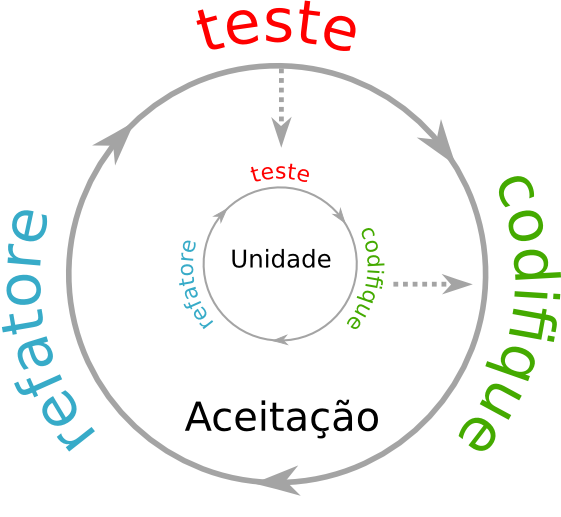
\includegraphics[scale=0.45]{images/ciclo-bdd}
  \label{img:ciclo-bdd}
\end{figure}

% subsection o_ciclo_bdd (end)

\subsection{Modelos de escrita dos testes de aceitação}
\label{sub:modelos_de_escrita_dos_testes_de_aceitacao}

Existem duas maneiras principais de se escrever os testes de aceitação: em texto plano e em código puro. Para exemplificar cada uma das abordagens, será especificada a seguinte funcionalidade:

\begin{quote}
\textit{Os comentários mostrados na página de tarefas devem ser renderizados utilizando a linguagem de marcação Markdown.}
\end{quote}

\subsubsection{Escrita em texto plano} % (fold)
\label{subsub:escrita_em_texto_plano}

Uma das maneiras de escrever testes de aceitação é como texto plano, em uma linguagem natural, ou seja, inglês, português e etc.

\citeonline{IntroducingBDD} estabelece um \textit{template} para a escrita para este tipo de especificação, sendo este uma captura dos critérios de aceitação de uma história:

\begin{quote}
\textbf{As a} (Como um) [X]\\
\textbf{I whant} (Eu quero) [Y]\\
\textbf{So that} (Para que) [Z]
\end{quote}

Onde Y é uma funcionalidade, Z é o benefício ou valor da funcionalidade e X é a pessoa (ou regra) que irá se beneficiar desta funcionalidade. O mapeamento feito desta forma é interessante pois se não souber completar Z, isso quer dizer que esta funcionalidade pode não ser tão importante quanto se imaginava.

Para finalizar esse \textit{template}, estes critérios de aceitação da história são quebrados em diferentes cenários que tem a seguinte forma:

\begin{quote}
\textbf{Given} (Dado) algum contexto inicial\\
\textbf{When} (Quando) algum evento ocorre\\
\textbf{Then} (Então) certifique-se de alguns resultados
\end{quote}

Nas ferramentas que implementam esta abordagem, os testes são escritos baseados em \textit{steps} (passos), onde cada \textit{step} (Given/When/Then) é mapeado para um código real.

No Código \ref{code:bdd_cucumber_spec}, é utilizado o \textit{Cucumber} para fazer a especificação. Como pode-se ver, o teste é escrito em linguagem que qualquer pessoa, mesmo sem nenhum conhecimento em programação, pode ler e validar.

\begin{mycode}{cucumber}%
{Especificação em texto plano}{code:bdd_cucumber_spec}
# features/comments.feature
Feature: Render comments with Markdown syntax
  As a user
  I want to use Markdown in my comments
  In order to make my comments more expressives

  Scenario: on tasks page
    Given I am a contributor of "sgtran" project
    And I am authenticated
    And I have a task of "sgtran" project
    When I am on the task page
    And I fill in "comment_content" with "# Some content [link](http://exemplo.com)"
    And I press "Comment"
    Then I should see "Some content" in a "h1" tag
    And I should see "link" in an "a" tag
\end{mycode}

Para cada \textit{step} existe uma implementação, ou seja, sua definição, chamada de \textit{step definition}. Pode-se pensar nos \textit{steps} como chamadas à métodos, e assim, os \textit{step definitions} serão as definição desse métodos. Deste modo, ao rodar os testes, o arquivo de teste é parseado e os \textit{steps} são executados.

Os \textit{step definitions} para os \textit{steps} do Código \ref{code:bdd_cucumber_spec} são apresentado no Código \ref{code:step_definition}. Como durante o desenvolvimento são escritos muitos \textit{step definitions}, com o intuito de organizá-los, eles são separados por contexto em diferentes arquivos.

\begin{mycode}{ruby}%
{Step definitions}{code:step_definition}
# features/step_definitions/contributor_steps.rb
Given /^I am a contributor of "([^"]*)" project$/ do |name|
  @project = Factory.create :project, :name => name
  @contributor = Factory.create :contributor, :contributions => [@project]
  @project.update_attribute(:contributors, [@contributor])
end

# features/step_definitions/contributor_steps.rb
Given /^I am(?:| an) authenticated(?:| contributor)$/ do
  @contributor ||= Factory.create :contributor

  Given %{I am on the sign in page}
  And %{I fill in "contributor_login" with "#{@contributor.email}"}
  And %{I fill in "contributor_password" with "#{@contributor.password}"}
  And %{I press "Sign in"}
end

# features/step_definitions/task_steps.rb
Given /^I have a task of "([^"]*)" project$/ do |project_name|
  @project = Factory.create :project, :name => 'project_name'
  @task = Factory.create :task, :project => @project, :author => @contributor
end

# features/step_definitions/web_steps.rb
Given /^(?:|I )am on (.+)$/ do |page_name|
  visit path_to(page_name)
end

# features/step_definitions/web_steps.rb
When /^(?:|I )fill in "([^"]*)" with "([^"]*)"$/ do |field, value|
  fill_in(field, :with => value)
end

# features/step_definitions/web_steps.rb
When /^(?:|I )press "([^"]*)"$/ do |button|
  click_button(button)
end

# features/step_definitions/my_web_steps.rb
When /^I should see "([^"]*)" in a(?:|n) "([^"]*)" tag$/ do |text, tag|
  if page.respond_to? :should
    page.should have_xpath("//#{tag}", :text => text)
  else
    assert page.has_xpath?("//#{tag}", :text => text)
  end
end
\end{mycode}

% subsubsection escrita_em_texto_plano (end)


\subsubsection{Escrita em código puro} % (fold)
\label{subsub:Escrita em codigo puro}

A outra maneira de escrever os testes de aceitação é com código puro. Nesta forma, todo o código dos testes (descrição e implementação) está concentrado em apenas um lugar, utilizando somente código para escrever os testes.

No Código \ref{code:bdd_spec1} pode-se ver a especificação em código puro para a funcionalidade.

\begin{mycode}{rspec}%
{Especificação em código puro}{code:bdd_spec1}
# spec/acceptance/comments_spec.rb
feature "Render comments with Markdown syntax" do
  background do
    @owner = Factory.create :contributor
    @project = Factory.create :project
    @task = Factory.create :task, :project => @project, :author => @owner
    login(@owner.email, @owner.password)
  end

  scenario "on tasks page" do
    visit project_task_path(@project, @task)
    fill_in "comment_content", :with => "# Some content [link](http://exemplo.com)"
    click_button "Comment"
    page.should have_xpath("//h1", :text => "Some content")
    page.should have_xpath("//a", :text => "link", :href => "http://exemplo.com")
  end
end
\end{mycode}

% subsubsection Escrita em codigo puro (end)

BDD vem se tornando um consenso em automação de testes. Contudo, existem uma divergência grande sobre a forma de escrita dos testes de aceitação entre escrita em código puro e escrita em texto plano, tendo alguns pontos a serem considerados.

\subsubsection{Legibilidade} % (fold)
\label{subsub:legibilidade}

Muitos defendem que os testes devem ser escritos em texto plano, por conta do teste ser escrito em linguagem que qualquer pessoa, mesmo sem nenhum conhecimento em programação, pode ler e validar.

Em uma situação onde se está desenvolvendo uma aplicação para um cliente, existe um mito sobre o cliente escrever as especificações, contudo está é uma abordagem utópica \cite{SteakOverCucumber, CucumberForVegetarians, ClientsWritingCucumber}. O cliente pode até ler e validar $-$ o que segundo \citeonline{YankoCapybara} nunca acontece $-$ mas mesmo assim esta não é uma abordagem muito interessante.

O cliente é especialista em problemas e os desenvolvedores em dar soluções. Se o cliente escreve a especificação, na realidade ele está escrevendo parte da solução \cite{SteakOverCucumber}. No caso da funcionalidade exemplificada anteriormente, o cliente apenas sabe que os ``comentários devem ser renderizados com markdown", ele não quer saber se para isso deve entrar em determinada página, preencher determinado campo e clicar em determinado botão. O cliente apenas sabe a funcionalidade que ele quer, e vê-la funcionando.

Dessa forma, o cliente não quer ler a especificação como no Código \ref{code:bdd_cucumber_spec}, nem validá-la, muito menos escrevê-la. Ele quer ler somente ``Render comments with Markdown syntax", mais do que isso é superficial \cite{WhyBotherWithCucumberTesting}; ele quer validar vendo funcionar e não quer escrever absolutamente nada.

Já em um contexto, como o do desenvolvimento do kanban-roots, no qual não existe um cliente, onde as pessoas que escrevem e leem as especificações são desenvolvedores, a escrita em texto plano tem um valor ainda menor. O código é uma linguagem natural para desenvolvedores, ainda mais quando é escrito em conjunto com DSLs\footnote{\textit{Domain specific language} (linguagem específica de domínio) é uma linguagem de programação de expressividade limitada, focada num domínio particular.} como a do Rspec \cite{SteakOverCucumber}.

% subsubsection legibilidade (end)

\subsubsection{Camada adicional} % (fold)
\label{subsub:camada_adicional}

Outra crítica aos testes em texto plano é que enquanto nos testes em código puro todo o código do teste está em concentrado em apenas um lugar, nos testes em texto plano, o código do testes está espalhado em diversos arquivos e métodos, devido a camada adicional dos \textit{steps}, tonando a suíte de testes mais complexa de manter e estender \cite{SteakOverCucumber}.

Além disso, é necessário manter um segundo ambiente de testes, já que para escrever os testes de aceitação em texto plano é necessária uma ferramenta de testes específica para isso. Isso não acontece com a escrita em código puro, já que é utilizada a mesma ferramenta utilizada nos testes unitários \cite{WhyBotherWithCucumberTesting}.

% subsubsection camada_adicional (end)

\subsubsection{Tempo de execução} % (fold)
\label{subsub:tempo_de_execucao}

Outro questionamento é sobre a velocidade para a execução dos testes. Como o \textit{Cucumber} utiliza a \textit{Gherkin}\footnote{\url{http://github.com/cucumber/cucumber/wiki/Gherkin}}, que é uma DSL externa\footnote{Uma DSL que tem sua própria sintaxe e necessita de um \textit{parser} para processá-la \cite{DSLFowler}.}, o arquivo de \textit{features} é parseado para que os \textit{steps} sejam executados, introduzindo um tempo extra na execução dos testes.

Para um conjunto de funcionalidades, foram escritos testes utilizando os ambos modelos de escrita $-$ apresentados no Anexo \ref{cha:codigo_do_comparativo}. Cada conjunto de vinte e dois exemplos foi executado separadamente e seus tempos de execução medidos, sendo os resultados apresentados na tabela \ref{table:tempo_de_execucao}.

\begin{table}[ht]
\caption{Velocidade de execução dos testes de acordo com o método de escrita}
\label{table:tempo_de_execucao}
\centering
\begin{tabular}{p{4.5cm} p{6.5cm}}
\toprule
\textbf{Método de escrita} & \textbf{Tempo médio de execução} \\
\midrule[1pt]
texto plano & 0m11.667s \\ \midrule
código puro & 0m8.8385s \\
\bottomrule
\end{tabular}
\end{table}

Analisando estes resultados pode-se concluir que os testes em código puro executam, em média, em um tempo 25\% menor que os em texto plano.

% subsubsection tempo_de_execucao (end)

\subsubsection{Um novo modelo de escrita} % (fold)
\label{ssub:um_novo_modelo_de_escrita}

\citeonline{YankoCapybara} propõe uma nova maneira de escrita de testes de aceitação, sendo esta uma união entre os duas maneiras apresentadas anteriormente. Os testes são escritos em código puro, porém utilizando \textit{steps} semelhantes aos do testes em texto plano. No código \ref{code:rspec_steps} é apresentado o exemplo anterior utilizando este novo modelo\footnote{Para a escrita deste exemplo, foi utilizada uma ferramenta criada por Yanko chamada \textit{Rspec example steps}. Mais em \url{https://github.com/railsware/rspec-example_steps}}.

\begin{mycode}{rspec}%
{Especificação mesclando código puro com texto plano}{code:rspec_steps}
feature "Render comments with Markdown syntax" do
  background do
    @owner = Factory.create :contributor
    @project = Factory.create :project
    @task = Factory.create :task, :project => @project, :author => @owner
    login(@owner.email, @owner.password)
  end

  Steps "Render on tasks page" do
    When "I am on the task page" do
      visit project_task_path(@project, @task)
    end
    And "I fill in the comment with an text with markdown syntax" do
      fill_in "comment_content", :with => "# Some content [link](http://exemplo.com)"
    end
    And "I press the Comment buttom" do
      click_button "Comment"
    end
    Then "I should see the text rendered as HTML" do
      page.should have_xpath("//h1", :text => "Some content")
      page.should have_xpath("//a", :text => "link", :href => "http://exemplo.com")
    end
  end
end
\end{mycode}

Esta abordagem busca eliminar os problemas com a camada adicional e tempo de execução que a escrita em texto plano têm. Alem disso, busca também aprimorar legibilidade da documentação da escrita em código puro, pois os testes, ao serem executados, produzem uma saída como mostrado na figura \ref{img:output-novo-modelo}

\begin{figure}[h]
  \center
  \caption{Saída produzida pela execução dos testes utilizando modelo proposto por Yanko}
  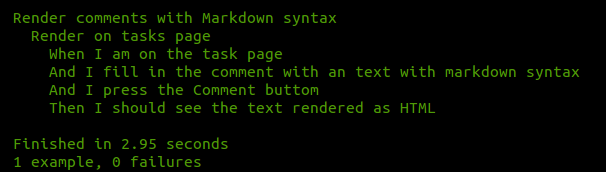
\includegraphics[scale=0.6]{images/output-novo-modelo}
  \label{img:output-novo-modelo}
\end{figure}

No entanto, esta abordagem cai no mesmo dilema da escrita em texto plano: o cliente não irá ler ou validar esta saída. Além disso, a introdução dos métodos \texttt{When/And/Then} juntamente com as \textit{strings} e blocos passados como parâmetros, piora muito a legibilidade do código de teste, prejudicando a manutenibilidade da suíte de testes. Assim, está abordagem, apesar de eliminar a camada adicional, pouco difere da escrita em texto plano, no que diz respeito às desvantagens.

% subsubsection um_novo_modelo_de_escrita (end)

\subsubsection{Conclusões} % (fold)
\label{subsub:conclusoes_bdd}

Na opinião do autor, os testes escritos em texto plano em um primeiro momento são muito atraentes, pois, com a facilidade de leitura, a possibilidade de validação de testes executáveis pelo cliente se tornam reais. No entanto, como apresentado anteriormente, na realidade é pouquíssimo provável que o cliente irá validar estes testes. Isto é ainda mais acentuado em projetos como o kanban-roots onde não existe cliente em si, tornando totalmente irrelevante os possíveis benefícios da escrita de testes em texto plano.

Já para projetos grandes, nos quais a suíte de testes é extensa, 25\% a mais no tempo de execução dos testes é um preço alto a ser pago, pois os testes devem ser executados diversas vezes ao dia. Se o tempo necessário para executar a suíte de testes se tornar demasiadamente longo, o desenvolvedor tende a rodar os testes menos vezes, diminuindo, assim, a eficácia da aplicação do BDD. Além disso, a escrita de testes em texto plano prejudica a produtividade, pois é adicionada complexidade ao processo, devido à camada adicional, fazendo com que a produtividade seja reduzida.

Apesar dos pontos negativos, os testes em texto plano podem ter valia em situações onde o desenvolvedor tem grandes dificuldades em entender o que o cliente quer ou entender o um determinado processo realizado pelo cliente. Desta forma, o teste em texto plano pode servir como um facilitador na comunicação. Assim, sentados lado a lado, o cliente vai dizendo ao desenvolvedor qual é o fluxo, e o desenvolvedor por sua vez, vai mapeando para o teste. Como ambos conseguem ler e entender o que está sendo escrito, a discussão e entendimento do problema é facilitada.

% subsubsection conclusoes_bdd (end)

% subsection modelos_de_escrita_dos_testes_de_aceitacao (end)

% section bdd (end)

\section{Integração contínua} % (fold)
\label{sec:integracao_continua}

Em uma equipe com vários desenvolvedores, todos trabalhando na elaboração de um mesmo sistema, existe o problema de unificar as diversas alterações feitas na base de código, assegurando que a base continua consistente \cite{ImproveitCI}. Para resolver esse problema, entra em cena a Integração Contínua (IC), que além disso, tem como ponto chave dar um feedback rápido quando a base de código não está consistente.

\cite{FowlerCI} definiu a IC da seguinte maneira:

\begin{citacao}
Integração Contínua é uma prática de desenvolvimento de software onde os membros de um time integram seu trabalho frequentemente, geralmente cada pessoa integra ao menos uma vez ao dia $-$ podendo haver múltiplas integrações por dia. Cada integração é verificada por um \textit{build} automatizado (incluindo testes) para detectar erros de integração o mais rápido possível. Muitos times acham que essa abordagem leva a uma significante redução nos problemas de integração e permite que um time desenvolva software coeso mais rapidamente. (tradução do autor)
\end{citacao}

Para assegurar o rápido feedback, o tempo de execução da \textit{build} deve ser o menor possível, tentando manter sempre menor do que dez minutos \cite{FowlerCI}.

Além disso, no servidor de integração, busca-se utilizar as mesmas configurações utilizadas em produção, pois em algumas situações os testes podem estar passando em ambiente de desenvolvimento, mas o \textit{bug} estourar em produção. O intuito é eliminar a famosa frase ``Mas funciona na minha máquina!".

A IC é um dos pilares da agilidade, pois garante que todo o sistema funcione de forma coesa a cada \textit{build}, mesmo que sua equipe seja grande e diversas partes do código estejam sendo alteradas ao mesmo tempo \cite{CaelumCI}.

Existem duas formas de executar a integração contínua: síncrona e assíncrona.

\subsection{Integração contínua síncrona} % (fold)
\label{sub:integracao_continua_sincrona}

Para a utilização da integração contínua síncrona, todos os desenvolvedores devem trabalhar no mesmo espaço físico, pois deve existir uma máquina dedicada à integração. Assim, apenas um desenvolvedor integra seu código de cada vez e outros só são liberados para integrar ao serem informados do término da integração corrente \cite{ImproveitCI}.

% subsection integracao_continua_assincrona (end)


\subsection{Integração contínua assíncrona} % (fold)
\label{sub:integracao_continua_assincrona}

Na integração contínua assíncrona, não existe a necessidade de todos os desenvolvedores trabalharem no mesmo espaço físico. Esse modelo é ideal para a maioria dos projetos open source, onde os desenvolvedores estão espalhados em diversas partes do mundo, pois em tais casos torna-se difícil ou impossível garantir que apenas um desenvolvedor irá integrar de cada vez \cite{ImproveitCI}.

Nesse modelo, o desenvolvedor deve assegurar que todos os testes estejam passando em sua máquina, e com essa condição atendida, pode integrar seu código ao repositório.

Além disso, um servidor de integração contínua, como o Jenkins\footnote{\url{http://jenkins-ci.org}} ou Travis\footnote{\url{http://travis-ci.org}}, deve monitorar o repositório permanentemente. Sempre que o servidor detecta modificações ele roda a \textit{build} e se encontra algum erro, envia um email para os desenvolvedores. Dessa forma, o desenvolvedor responsável deve fazer as correções o mais brevemente possível e enviá-las para o repositório.

% subsection integracao_continua_sincrona (end)

\subsection{Integração contínua síncrona x assíncrona} % (fold)
\label{sub:sincrona_x_assincrona}

Sempre que possível, o melhor modelo de integração a ser utilizado é o síncrono. Pode-se fazer essa afirmação baseado no que \citeonline{ArtOfAgileDevelopment} descrevem como vantagens em utilizar a integração contínua síncrona:

\begin{itemize}
  \item Se a \textit{build} falhar, não é necessário interromper uma nova tarefa iniciada para voltar e corrigir a anterior, evitando assim a mudança de contexto mental.
  \item Ajuda a manter a \textit{build} rápida, pois se está levando muito tempo para executar, a percepção é imediata e pode ser logo corrigida.
  \item A frequência de \textit{builds} quebradas é muito menor, assim o tempo de permanência da falha no sistema de controle de versão, pois o responsável pela modificação que introduziu a falha pode não estar apto para corrigir-la imediatamente.
\end{itemize}

\citeonline{ImproveitCI} corrobora dizendo o seguinte:

\begin{citacao}
A integração contínua assíncrona permite o trabalho de desenvolvedores distribuídos geograficamente, porém é um pouco mais arriscada e menos eficiente que a integração síncrona. O risco aumenta porque o repositório pode ficar inconsistente durante alguns períodos de tempo $-$ sempre que um erro ocorre e o responsável por ele ainda não fez o commit das correções.

Na integração assíncrona, a eficiência diminui porque leva mais tempo para o desenvolvedor descobrir que cometeu um erro. É comum o desenvolvedor receber a notificação de um erro depois de já ter iniciado uma nova atividade. Ao ser notificado, deve parar a nova tarefa, relembrar o que havia feito na tarefa anteriormente e corrigir o erro.

O processo síncrono é mais eficiente no uso do feedback exatamente porque impede o desenvolvedor de desviar sua atenção para qualquer outra atividade, enquanto a integração não tiver sido concluída com sucesso.
\end{citacao}

% subsection sincrona_x_assincrona (end)

\subsection{Integração contínua no kanban-roots} % (fold)
\label{sub:integracao_continua_no_kanban}

Com base no tópico anterior e por ser um projeto \textit{open source}, no kanban-roots foi utilizado o método assíncrono de integração contínua, através do Travis\footnote{Mais informações podem ser encontradas em \url{http://travis-ci.org}}, que foi escolhido por ser um serviço hospedado integração contínua para a comunidade open source, o que facilitou bastante pela não necessidade de manutenção de uma estrutura local de integração contínua.

A integração contínua se mostrou importante em algumas ocasiões durante o desenvolvimento do kanban-roots, a exemplo:

\begin{itemize}
  \item Alguns arquivos não foram incluídos no commit, fazendo com que localmente tudo funcionasse perfeitamente, mas o repositório estava quebrado.
  \item Em ambiente de desenvolvimento é utilizado o SQLite\footnote{\url{http://www.sqlite.org}} e em ambiente de produção, é utilizado o MySQL\footnote{\url{http://www.mysql.com}}. Assim, foi feita uma query que apenas funcionava no SQLite, mas não no MySQL. Ou seja, em desenvolvimento estava perfeito, mas em produção, não.
\end{itemize}

Com o feedback rápido, todas as falhas foram corrigidas muito rapidamente, sem que problemas maiores ocorressem.

% subsection integracao_continua_no_kanban (end)

% section integracao_continua (end)


\section{Dublês de Teste} % (fold)
\label{sec:dubles_de_teste}

Em algumas ocasiões é difícil testar alguns componentes porque eles dependem de outros componentes que não podem ser utilizados em ambiente de teste. Estas situações podem acontecer por esses componentes não estarem disponíveis, por eles não retornarem os resultados necessários ou porque executá-los iria trazer efeitos colaterais indesejados. Em outros casos, a estratégia de testes utilizada requer que se tenha mais controle do comportamento interno do componente.

Quando se escreve um teste onde não se pode/escolhe usar componentes reais, pode-se substitui-los pelos Dublês de Teste que oferecem uma maneira de isolar as dependências ao criar os testes, permitindo a utilização de componentes falsos para cumprir os papéis de componentes reais. Com isso, elimina-se complexidade do código dos testes, pois o código de implementação dos objetos é mantido pequeno e com baixo acoplamento.

Os Dublês de Teste não precisam se comportar exatamente como o componente real, devendo apenas prover a mesma API que o componente real.

\citeonline{XUnit} define cinco categorias de Dublês de Teste:

\begin{itemize}
\item
Objetos \textbf{\textit{Dummy}} geralmente são utilizados apenas para preencher uma lista de parâmetros e nunca são realmente usados.

TODO: Sobre dummies nunca serem realmente usados, dá uma olhada na abordagem do Ludibrio https://github.com/nsigustavo/ludibrio.

\item
Objetos \textbf{\textit{Fake}} são utilizados para substituir funcionalidades reais de um componente por razões diferentes de verificações indiretas de entradas e saídas do componente a ser testado. TODO: Explique as razões.

\item
Os \textbf{\textit{Stubs}} provêm respostas prontas para chamadas feitas durante os testes, geralmente não respondendo a qualquer   chamada diferente
das pré-definidas.

\item
Os \textbf{\textit{Spies}} são \textit{Stubs} que também tem gravam algumas informações baseadas em como eles são chamados. Um exemplo   pode ser um serviço de email que grava quantas mensagens foram   enviadas.

\item
\textbf{\textit{Mocks}} são objetos pré-programados para receber determinado conjunto de chamadas, podendo lançar uma exceção se tais chamadas não forem feitas a ele, ou se receber outra chamada diferente das pré-programadas.

referência: the art of agile development, página 298.
\end{itemize}

De modo geral, a utilização de Dublês de Teste é extremamente benéfica para o projeto. Contudo, existem controvérsias, principalmente em relação a utilização do \textit{Mock} \cite{MocksArentStubs}. TODO: Entrar na controvérsia.

% section dubles_de_teste (end)

